\chapter{El universo newtoniano en expansión}

\lectureoverview{La cosmología moderna comienza cuando se trata al universo mismo como un sistema físico. Partiendo de la isotropía y la homogeneidad a gran escala, introducimos una retícula comóvil y codificamos su movimiento mediante un único factor de escala \(a(t)\). El teorema de las capas esféricas de Newton reduce entonces el problema gravitatorio de muchos cuerpos a una ecuación para \(a(t)\). La conservación de la energía distingue entre universos que vuelven a colapsar, críticos y en expansión eterna; el caso crítico dominado por materia proporciona la primera ecuación de Friedmann y la ley \(a(t)\propto t^{2/3}\).}

\section{Cuando la cosmología se convirtió en física}

La cosmología es una disciplina antigua, pero la cosmología cuantitativa es joven. Para nuestros fines, no hace falta empezar por los griegos. Los puntos de partida históricos útiles son el descubrimiento de la expansión cósmica por Hubble en el segundo cuarto del siglo XX y, más tarde, el reconocimiento del fondo de microondas, de unos tres kelvin, como vestigio de un universo temprano caliente.

Antes de que las mediciones alcanzaran precisión, buena parte de la astronomía se parecía necesariamente a la historia natural. Se encontraba una estrella inusual, se clasificaba una galaxia peculiar, se medía lo que se podía medir y se elaboraba un catálogo de objetos. Esos objetos eran, desde luego, sistemas físicos: tenían momento angular, contenían elementos químicos y obedecían las leyes de la mecánica. El cambio decisivo consistió en tratar el \emph{universo entero} como un sistema físico único, regido por ecuaciones lo bastante precisas para contrastarlas con las observaciones.

Ese es el tema de este capítulo. No nos limitaremos a enumerar el contenido del universo; preguntaremos cuáles son sus variables, cómo se mueve y cuál es su ley dinámica. Las ecuaciones no son un adorno que se añade después a la cosmología. Son el medio por el que el universo se convierte en un problema de física.

Históricamente, el universo en expansión se comprendió en el lenguaje de la relatividad general. Sin embargo, desde el punto de vista lógico, buena parte del argumento inicial es newtoniano. Un físico del siglo XVII que hubiera conjeturado el movimiento correcto a gran escala podría haber derivado un modelo extraordinariamente bueno. Empezar con Newton no pretende sustituir la relatividad, sino poner de manifiesto la mecánica que esta reorganiza después en términos geométricos.

\section{Isotropía, homogeneidad y principio cosmológico}

El primer paso es observacional. A escalas suficientemente grandes, el universo es aproximadamente \emph{isótropo}: después de promediar sobre regiones del cielo y mirar más allá del primer plano de la Vía Láctea, presenta un aspecto muy parecido en todas las direcciones. Esto no significa que sea exactamente uniforme. Mirar directamente una estrella cercana no es lo mismo que mirar una región vacía, y la distribución de materia contiene estructuras reales. La isotropía es una afirmación promediada a gran escala.

La homogeneidad es una afirmación distinta. Significa que el universo promediado es igual de un lugar a otro. Un observador situado a muchas galaxias de distancia debería ver, tras realizar el mismo promedio a gran escala, aproximadamente el mismo tipo de universo que vemos nosotros.

En una primera aproximación, una galaxia puede tratarse simplemente como un punto material. El universo visible contiene aproximadamente
\begin{equation}
N_{\rm gal}\sim 10^{11}
\end{equation}
galaxias, cada una con del orden de \(10^{11}\) estrellas. Esto da aproximadamente \(10^{22}\) estrellas. Si se toma, como estimación deliberadamente aproximada del orden de magnitud, diez planetas por estrella, se obtienen \(10^{23}\) planetas, una cantidad curiosamente cercana a un mol de planetas. Esta estimación numérica no forma parte de la dinámica, pero fija la escala del sistema que idealizamos.

\begin{classroomqa}
\classquestion{¿Cuántas galaxias hay en el universo observable, aproximadamente, en orden de magnitud?}
\lecturerresponse{Unos cien mil millones, es decir, \(10^{11}\). Con aproximadamente \(10^{11}\) estrellas por galaxia, eso significa que hay alrededor de \(10^{22}\) estrellas en el universo visible. Conviene tener presentes estas estimaciones de escala, aunque en el cálculo siguiente reemplacemos cada galaxia por un único punto material. \lecturetimestamp{00:06:08--00:07:05}}
\end{classroomqa}

¿Por qué la isotropía a nuestro alrededor debería sugerir homogeneidad? Imaginemos una distribución isótropa que \emph{no} sea homogénea. Su densidad tendría que variar con la distancia respecto de nosotros, pero no con la dirección: en efecto, formaría un patrón de capas concéntricas centradas en nuestra posición. Un observador desplazado respecto del centro común ya no vería isotropía. Por tanto, hay dos posibilidades:
\begin{enumerate}
\item ocupamos un centro privilegiado en torno al cual se ha dispuesto el universo; o
\item la distribución a gran escala es aproximadamente homogénea y, por tanto, ningún punto ocupado es privilegiado.
\end{enumerate}
La segunda posibilidad es la más económica. La isotropía, junto con la negativa a atribuirnos una posición cósmica privilegiada, conduce a la homogeneidad.

\begin{classroomqa}
\classquestion{¿Qué forma podría tener una distribución isótropa, pero no homogénea?}
\lecturerresponse{Su variación podría depender solo de la distancia respecto de nosotros, formando un patrón de capas centrado en nuestra posición. Si el observador se aleja de ese centro, el patrón deja de ser isótropo. Por tanto, a menos que nuestra ubicación sea especial, la isotropía apunta a la homogeneidad. \lecturetimestamp{00:07:06--00:08:54}}
\end{classroomqa}

La hipótesis conjunta se denomina \emph{principio cosmológico}: a escalas suficientemente grandes, el universo es espacialmente homogéneo e isótropo. Llamarlo principio no lo demuestra. Históricamente, los cosmólogos adoptaron esta hipótesis antes de que las observaciones la justificaran con solidez. Su validez se basa en su éxito empírico.

Tampoco la homogeneidad es exacta. Las galaxias forman cúmulos y supercúmulos, y desde hace tiempo se debate la existencia de estructuras que abarcan fracciones muy grandes del cielo visible. La afirmación adecuada es que las fluctuaciones se promedian y desaparecen cuando la región de promediado es suficientemente grande---del orden de cientos de millones hasta aproximadamente mil millones de años luz en esta introducción. Las observaciones pueden precisar esa escala; el método consiste en promediar a escalas cada vez mayores hasta que la estructura local deje de dominar la descripción.

\begin{classroomqa}
\audiencequestion{¿La uniformidad del fondo cósmico de microondas aporta pruebas a favor del principio cosmológico?}
\lecturerresponse{Sí. El principio cosmológico se propuso antes de que hubiera una base observacional sólida para sostenerlo, pero más tarde el fondo de microondas mostró que el universo primordial era extraordinariamente uniforme. Las galaxias y los cúmulos surgieron de pequeñas desviaciones respecto de ese estado uniforme; no borran las pruebas de su uniformidad a gran escala. \lecturetimestamp{00:10:53--00:11:43}}
\end{classroomqa}

\section{Una retícula que se mueve con las galaxias}

Una vez elegida la aproximación observacional, debemos elegir las variables. A la pregunta «¿Cuál es el primer paso para plantear un problema de física?», una respuesta de aula es conocer las variables; la respuesta tradicional es afilar el lápiz. Aquí, la variable importante se obtiene eligiendo bien las coordenadas.

Imaginemos una retícula tridimensional con etiquetas \(x,y,z\). Estas etiquetas no tienen por qué representar distancias medidas en metros. Son números de coordenadas. Elegimos la retícula de modo que, una vez promediados los pequeños movimientos peculiares, cada galaxia permanezca en un punto fijo de la retícula. Las galaxias son entonces \emph{comóviles}.

Esta elección sería inútil si las galaxias se movieran al azar. Sin embargo, las observaciones revelan un movimiento coherente a gran escala. Las celdas vecinas de la retícula pueden expandirse o contraerse, pero la misma expansión o contracción ocurre en todas partes. Por tanto, todas las distancias físicas pueden expresarse como un factor común dependiente del tiempo multiplicado por una separación de coordenadas fija.

Para dos galaxias \(A\) y \(B\),
\begin{equation}
\begin{aligned}
d_{AB}(t)&=a(t)\,\Delta\chi_{AB},\\
\Delta\chi_{AB}
&=\sqrt{(x_A-x_B)^2+(y_A-y_B)^2+(z_A-z_B)^2}.
\end{aligned}
\label{eq:c01-physical-distance}
\end{equation}
Si difieren solo en la coordenada \(x\), esto se reduce a
\begin{equation}
d_{AB}(t)=a(t)\,\Delta x_{AB}.
\end{equation}
La función \(a(t)\) es el \emph{factor de escala}. Su normalización absoluta es convencional: multiplicar todas las coordenadas comóviles por una constante y dividir \(a\) por esa misma constante no cambia ninguna distancia física. Las razones como \(a(t_2)/a(t_1)\), y las derivadas divididas por \(a\), contienen la información física.

Derivemos la ecuación~\eqref{eq:c01-physical-distance}. La separación comóvil es fija, de modo que
\begin{equation}
v_{AB}=\dot a\sqrt{(\Delta x)^2+(\Delta y)^2+(\Delta z)^2}.
\end{equation}
Al dividir por la distancia física, obtenemos
\begin{equation}
\frac{v_{AB}}{d_{AB}}=\frac{\dot a}{a}\equiv H(t),
\label{eq:c01-hubble-parameter}
\end{equation}
o bien
\begin{equation}
\boxed{v_{AB}=H(t)d_{AB}.}
\label{eq:c01-hubble-law}
\end{equation}
Esta es la ley de Hubble para el flujo homogéneo ideal.

El nombre «constante de Hubble» puede inducir a error. En un instante cósmico dado, el mismo valor de \(H\) se aplica en todos los puntos del modelo homogéneo, pero \(H(t)\) en general cambia con el tiempo. La universalidad espacial no implica constancia temporal.

\begin{classroomqa}
\audiencequestion{Al expresar todas las distancias como un único \(a(t)\) común multiplicado por una separación de coordenadas fija, ¿hemos supuesto ya la ley de Hubble?}
\lecturerresponse{La hipótesis está sin duda motivada por la observación de Hubble; no se nos habría ocurrido sin pruebas de una recesión coherente. Su utilidad consiste en organizar esas pruebas. En vez de asignar una velocidad independiente a cada galaxia, describimos una única retícula en expansión. Una vez adoptada esa descripción, la proporcionalidad \(v=Hd\) se obtiene al derivar. \lecturetimestamp{00:24:20--00:25:33}}
\end{classroomqa}

El mismo movimiento admite dos descripciones verbales. Podemos decir que las galaxias se alejan unas de otras a través del espacio, o que permanecen en posiciones comóviles fijas mientras la retícula---y, por tanto, el espacio físico entre ellas---se expande. En esta etapa, son dos descripciones coordinadas de la misma matemática. La relatividad general hará especialmente natural el lenguaje del espacio en expansión, pero ninguna observación puede distinguir dos descripciones que asignen las mismas separaciones físicas en todo instante.

\section{Balance de masa en una celda comóvil}

Antes de introducir la gravedad, llevemos la cuenta de la masa. Consideremos una pequeña celda de coordenadas cuyo volumen es
\begin{equation}
\Delta V_{\rm com}=\Delta x\,\Delta y\,\Delta z.
\end{equation}
Aun así, debe ser lo bastante grande para contener muchas galaxias, de modo que puedan promediarse las fluctuaciones locales. Sea \(\nu\) la masa por unidad de volumen de coordenadas comóviles. La masa de la celda es
\begin{equation}
\Delta M=\nu\,\Delta x\,\Delta y\,\Delta z.
\label{eq:c01-comoving-mass}
\end{equation}
Como la celda se mueve con la materia, ninguna galaxia cruza su frontera en el flujo ideal, y \(\Delta M\) es constante.

Cada arista física es más larga que la correspondiente arista de coordenadas por un factor \(a(t)\). Por tanto, el volumen físico es
\begin{equation}
\Delta V_{\rm phys}=a^3(t)\,\Delta x\,\Delta y\,\Delta z.
\end{equation}
La densidad de masa física es
\begin{equation}
\boxed{\rho(t)=\frac{\Delta M}{\Delta V_{\rm phys}}=\frac{\nu}{a^3(t)}.}
\label{eq:c01-density-dilution}
\end{equation}
La expansión diluye la materia sin presión según \(a^{-3}\); la contracción la concentra de acuerdo con la misma ley.

Hasta aquí no hemos supuesto nada sobre la dinámica. Hemos usado geometría euclídea, una hipótesis cinemática y la conservación de la masa en una celda comóvil. Ahora entra en juego la gravedad.

\section{Entra Newton}

Una imagen tentadora, pero incorrecta, sostiene que una distribución infinita y uniforme de materia debería permanecer estática porque la atracción de un lado queda compensada por la del otro. El defecto es que esta compensación informal no proporciona una ecuación coherente para la aceleración relativa. El teorema de las capas esféricas de Newton organiza correctamente la fuerza.

Elijamos cualquier galaxia como origen \(O\) y consideremos una galaxia \(A\) a un radio comóvil fijo
\begin{equation}
R=\sqrt{x^2+y^2+z^2}.
\end{equation}
Su radio físico, velocidad radial y aceleración radial son
\begin{equation}
d=aR,
\qquad
\dot d=\dot a R,
\qquad
\ddot d=\ddot a R.
\label{eq:c01-radial-kinematics}
\end{equation}

\begin{figure}[ht]
\centering
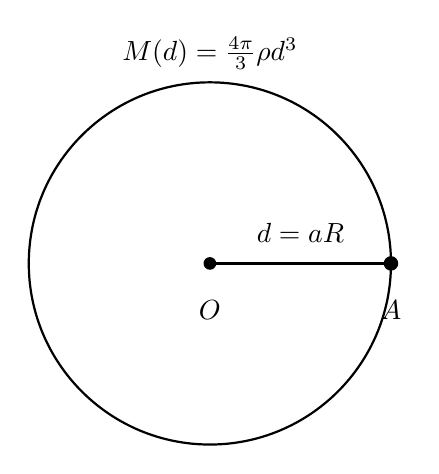
\begin{tikzpicture}[scale=1.15]
\draw[thick] (0,0) circle (2);
\fill (0,0) circle (0.07);
\fill (2,0) circle (0.08);
\draw[thick] (0,0) -- (2,0);
\draw (1,0.12) node[above] {\(d=aR\)};
\draw (0,-0.3) node[below] {\(O\)};
\draw (2,-0.3) node[below] {\(A\)};
\draw (0,2.32) node {\(M(d)=\frac{4\pi}{3}\rho d^3\)};
\end{tikzpicture}
\caption{La reducción newtoniana. Para calcular la aceleración de la galaxia \(A\), las capas exteriores se cancelan y la masa dentro del radio \(d\) actúa como si estuviera concentrada en \(O\).}
\label{fig:c01-newton-sphere}
\end{figure}

En una distribución de masa esféricamente simétrica, la fuerza neta debida a la materia situada fuera de la esfera que pasa por \(A\) es nula. La materia interior actúa como si estuviera concentrada en el centro. La masa encerrada es
\begin{equation}
M(d)=\frac{4\pi}{3}\rho d^3.
\label{eq:c01-enclosed-mass}
\end{equation}
La ley de la inversa del cuadrado de Newton da entonces la aceleración de \(A\):
\begin{equation}
\ddot d=-\frac{GM(d)}{d^2}.
\end{equation}
Usando la ecuación~\eqref{eq:c01-radial-kinematics},
\begin{align}
\ddot a R
&=-\frac{G}{d^2}\left(\frac{4\pi}{3}\rho d^3\right) \\
&=-\frac{4\pi G}{3}\rho d \\
&=-\frac{4\pi G}{3}\rho aR.
\end{align}
El radio comóvil se cancela y queda
\begin{equation}
\boxed{\frac{\ddot a}{a}=-\frac{4\pi G}{3}\rho.}
\label{eq:c01-acceleration}
\end{equation}
Esta cancelación es la prueba de coherencia. Todas las galaxias comóviles, cualquiera que sea \(R\), obedecen la misma ecuación para un mismo factor de escala.

Al sustituir la ecuación~\eqref{eq:c01-density-dilution}, obtenemos cualquiera de las dos formas equivalentes
\begin{equation}
\frac{\ddot a}{a}=-\frac{4\pi G\nu}{3a^3},
\qquad
\ddot a=-\frac{4\pi G\nu}{3a^2}.
\label{eq:c01-acceleration-nu}
\end{equation}
La primera forma muestra la aceleración fraccionaria; la segunda aísla \(\ddot a\). Dejar \(a\) en el miembro izquierdo es una convención, no un cambio en la física.

\begin{classroomqa}
\audiencequestion{El origen era arbitrario, pero todas las fuerzas del cálculo apuntan hacia él. ¿Cómo puede otro origen dar el mismo universo?}
\lecturerresponse{La ecuación describe el movimiento relativo. Si repetimos el cálculo alrededor de cualquier otra galaxia, obtenemos la misma ecuación porque, por homogeneidad, la masa encerrada depende solo del radio físico. Si pasamos a un sistema acelerado ligado a otra galaxia, pero mantenemos las fuerzas referidas al primer origen, también debemos incluir la fuerza inercial correspondiente. Elegir un sistema de referencia en reposo en el centro simplemente evita ese cálculo adicional. El resultado invariante es la ecuación~\eqref{eq:c01-acceleration}, no la existencia de un centro privilegiado. \lecturetimestamp{00:43:56--00:46:58}}
\end{classroomqa}

\begin{classroomqa}
\audiencequestion{¿Se mantendría el resultado si la densidad de masa comóvil \(\nu\) variara de un lugar a otro?}
\lecturerresponse{No con esta forma de una sola función. La cancelación sencilla depende de que \(M\propto d^3\) mantenga la misma proporcionalidad en todas partes. Si \(\nu\) variara apreciablemente a lo largo de la escala de promediado, distintas regiones necesitarían dinámicas locales distintas y un único factor de escala homogéneo ya no las describiría. La homogeneidad cumple una función esencial. \lecturetimestamp{00:47:05--00:47:51}}
\end{classroomqa}

\begin{classroomqa}
\audiencequestion{¿Por qué escribir \(\ddot a/a\) en vez de pasar el factor \(a\) al miembro derecho?}
\lecturerresponse{Las dos formas son correctas. En cosmología se suele escribir la aceleración fraccionaria \(\ddot a/a\), en parte porque se puede comparar directamente con la tasa de expansión fraccionaria \(H=\dot a/a\). Al multiplicar por \(a\) se obtiene la misma ecuación diferencial. \lecturetimestamp{00:50:36--00:51:29}}
\end{classroomqa}

La ecuación~\eqref{eq:c01-acceleration} descarta de inmediato un universo newtoniano homogéneo y estático lleno de materia ordinaria. Un factor de escala estático tendría \(\ddot a=0\), mientras que una densidad positiva hace que el miembro derecho sea negativo. Esto \emph{no} nos dice todavía si el universo está en expansión o en contracción. Solo nos indica el signo de la aceleración.

\section{Aceleración negativa no significa contracción}

La distinción entre velocidad y aceleración es elemental, pero decisiva. Un Ferrari que avanza por una autopista alemana puede tener velocidad positiva mientras frena con aceleración negativa. De igual modo, un universo puede cumplir
\begin{equation}
\dot a>0,
\qquad
\ddot a<0:
\end{equation}
está en expansión, pero esta se ralentiza.

Para determinar si el movimiento acabará invirtiéndose, comparemos el problema cosmológico con el de una partícula de prueba que se mueve radialmente en el campo gravitatorio terrestre. Sea \(x\) ahora la distancia física de la partícula a una masa central \(M\); no tiene relación con la coordenada comóvil anterior. La ecuación de Newton es
\begin{equation}
\ddot x=-\frac{GM}{x^2}.
\label{eq:c01-particle-force}
\end{equation}
La aceleración siempre apunta hacia dentro. Sin embargo, una partícula lanzada hacia fuera puede seguir moviéndose en esa dirección durante mucho tiempo, o para siempre. Una partícula que ya se mueve hacia dentro adquiere una velocidad cada vez más negativa. La ley de fuerza por sí sola no determina cuál de estos movimientos ocurre; eso depende de las condiciones iniciales.

\begin{classroomqa}
\audiencequestion{¿Significa \(\ddot a<0\) que el universo se está contrayendo?}
\lecturerresponse{No. La contracción significa \(\dot a<0\). Que \(\ddot a\) sea negativa solo significa que \(\dot a\) disminuye con el tiempo. Si \(\dot a\) comienza siendo positiva, la gravedad ralentiza la expansión; que llegue o no a cero depende de la velocidad de expansión inicial, igual que el destino de un proyectil lanzado hacia fuera depende de que su velocidad sea menor o mayor que la velocidad de escape. \lecturetimestamp{00:51:30--00:56:18}}
\end{classroomqa}

\begin{figure}[ht]
\centering
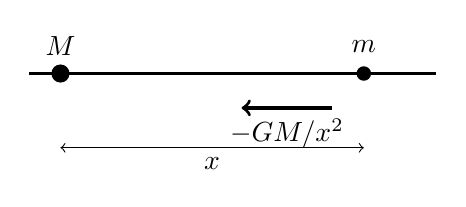
\begin{tikzpicture}[scale=1.15]
\fill (0,0) circle (0.1);
\draw (0,0.3) node {\(M\)};
\draw[thick] (-0.35,0) -- (4.15,0);
\fill (3.35,0) circle (0.08);
\draw (3.35,0.3) node {\(m\)};
\draw[->,very thick] (3.0,-0.38) -- (2.0,-0.38)
  node[midway,below] {\(-GM/x^2\)};
\draw[<->] (0,-0.82) -- (3.35,-0.82)
  node[midway,below] {\(x\)};
\end{tikzpicture}
\caption{El problema radial de una partícula se utilizó para separar el signo de la aceleración de la dirección y el destino del movimiento.}
\label{fig:c01-particle-sketch}
\end{figure}

La energía hace evidentes las distintas posibilidades. La energía mecánica conservada es
\begin{equation}
E=\frac12 m\dot x^{\,2}-\frac{GMm}{x}.
\label{eq:c01-particle-energy}
\end{equation}
La energía potencial es proporcional a \(1/x\), no a \(1/x^2\); al derivar \(-GMm/x\) se obtiene la fuerza de la inversa del cuadrado.

\begin{figure}[ht]
\centering
\includegraphics[width=0.82\textwidth]{lecture_01_figure_02.png}
\caption{La pizarra al inicio del argumento energético: una masa de prueba en movimiento y su término cinético, justo antes de volver a incluir la energía potencial gravitatoria.}
\lectureframe{00:58:57}
\end{figure}

Si \(E<0\), una partícula que se mueve hacia fuera no puede llegar al infinito, donde su energía potencial tiende a cero y su energía cinética es no negativa. Debe detenerse en un valor finito de \(x\) y regresar. Si \(E>0\), no puede detenerse, porque en un punto de retorno la energía cinética se anularía y la energía potencial restante sería negativa, en contradicción con la conservación de una \(E\) positiva. La frontera es
\begin{equation}
E=0,
\end{equation}
que define la velocidad de escape:
\begin{equation}
\frac12 m v_{\rm esc}^2-\frac{GMm}{x}=0,
\qquad
\boxed{v_{\rm esc}^2=\frac{2GM}{x}.}
\label{eq:c01-escape-velocity}
\end{equation}

\begin{figure}[ht]
\centering
\includegraphics[width=0.88\textwidth]{lecture_01_figure_03.png}
\caption{La frontera de energía nula va tomando forma en la pizarra. Las ecuaciones cosmológicas de aceleración anteriores siguen encuadradas a la izquierda mientras se desarrolla a la derecha el problema radial de escape.}
\lectureframe{01:01:37}
\end{figure}

Justo a la velocidad de escape, la partícula se ralentiza indefinidamente. Su rapidez tiende a cero solo cuando \(x\to\infty\); nunca alcanza un punto de retorno a distancia finita. Este caso límite será el modelo cosmológico más sencillo.

\section{La ecuación cosmológica de la energía}

Volvamos a una galaxia situada a un radio comóvil fijo \(R\). Por el teorema de las capas esféricas, su movimiento radial es idéntico al de una partícula que se desplaza en el exterior de una masa puntual igual a la masa encerrada por su esfera comóvil.

\begin{figure}[ht]
\centering
\includegraphics[width=0.82\textwidth]{lecture_01_figure_04.png}
\caption{La fuerza de la inversa del cuadrado y el esquema de la partícula radial que se usan al trasladar a la cosmología el argumento energético de una sola partícula.}
\lectureframe{01:04:14}
\end{figure}

La masa encerrada no aumenta cuando la esfera física se expande. La esfera es comóvil, por lo que siempre contiene las mismas galaxias:
\begin{align}
M
&=\frac{4\pi}{3}\rho(aR)^3 \\
&=\frac{4\pi}{3}\frac{\nu}{a^3}a^3R^3 \\
&=\frac{4\pi}{3}\nu R^3.
\label{eq:c01-fixed-enclosed-mass}
\end{align}
La primera expresión solo parece depender del tiempo hasta que se tiene en cuenta la dilución de la densidad. Los factores de \(a^3\) se cancelan.

\begin{classroomqa}
\audiencequestion{Al expandirse la esfera, ¿encierra más masa?}
\lecturerresponse{No. Su radio físico crece, pero su frontera comóvil se mueve con las galaxias. En el flujo homogéneo ideal, ninguna materia cruza esa frontera, y la ecuación~\eqref{eq:c01-fixed-enclosed-mass} muestra explícitamente la cancelación. \lecturetimestamp{01:04:37--01:05:20}}
\end{classroomqa}

La velocidad física de la galaxia es \(\dot d=\dot a R\) y su distancia al origen elegido es \(d=aR\). Por tanto, su energía newtoniana conservada es
\begin{equation}
\boxed{
E=\frac12 m\dot a^{\,2}R^2-\frac{GMm}{aR}.
}
\label{eq:c01-cosmological-energy}
\end{equation}

\begin{figure}[ht]
\centering
\includegraphics[width=0.82\textwidth]{lecture_01_figure_05.png}
\caption{Los términos cinético y potencial cosmológicos en la pizarra. El denominador completo \(aR\) de la ecuación~\eqref{eq:c01-cosmological-energy} se obtiene a partir del radio físico y de la derivación correspondiente.}
\lectureframe{01:06:12}
\end{figure}

Los tres casos de energía de la partícula corresponden a tres casos cosmológicos:
\begin{description}[style=nextline]
\item[\(E<0\):] la expansión inicial está por debajo de la velocidad de escape; \(a(t)\) alcanza un máximo y el universo vuelve a colapsar.
\item[\(E=0\):] el universo es exactamente crítico; la expansión se ralentiza para siempre y la velocidad se aproxima asintóticamente a cero.
\item[\(E>0\):] la expansión inicial supera la velocidad de escape; en el modelo newtoniano, el universo se expande para siempre con una velocidad de recesión asintótica distinta de cero.
\end{description}

Empezamos por el caso límite \(E=0\). Igualamos a cero la ecuación~\eqref{eq:c01-cosmological-energy}, cancelamos \(m\) y dividimos por \(a^2R^2/2\), lo cual da
\begin{align}
\frac12\dot a^{\,2}R^2&=\frac{GM}{aR}, \\
\left(\frac{\dot a}{a}\right)^2&=\frac{2GM}{a^3R^3}.
\label{eq:c01-energy-intermediate}
\end{align}
Como
\begin{equation}
\rho=\frac{M}{(4\pi/3)a^3R^3},
\end{equation}
la ecuación~\eqref{eq:c01-energy-intermediate} se convierte en
\begin{equation}
\boxed{
H^2=\left(\frac{\dot a}{a}\right)^2=\frac{8\pi G}{3}\rho.
}
\label{eq:c01-first-friedmann}
\end{equation}
Esta es la primera ecuación de Friedmann para un universo espacialmente plano, compuesto solo por materia y con constante cosmológica nula, obtenida aquí a partir de la conservación newtoniana de la energía.

\begin{classroomqa}
\classquestion{¿Qué le ocurre a una partícula lanzada exactamente a la velocidad de escape?}
\lecturerresponse{Se ralentiza sin llegar a invertir su movimiento. Su velocidad se aproxima a cero solo a distancia infinita. El universo de energía nula se comporta del mismo modo: \(H\) disminuye, pero \(\dot a\) sigue siendo positiva y no hay un cambio de sentido en tiempo finito. \lecturetimestamp{01:10:45--01:12:10}}
\end{classroomqa}

Los factores \(4\pi/3\) y \(8\pi G/3\) no son adornos arbitrarios. \(4\pi/3\) es el volumen de una esfera, y el factor dos procede de la energía cinética. En relatividad general, el mismo factor \(8\pi G\) aparece en la ecuación de campo de Einstein, y su componente temporal conduce a la ecuación relativista de Friedmann. Esta concordancia no es accidental, pero la derivación presente todavía no incluye la presión, la curvatura espacial como geometría ni una constante cosmológica.

\section{La solución crítica dominada por materia}

Usemos la ley de densidad \(\rho=\nu/a^3\) en la ecuación~\eqref{eq:c01-first-friedmann}:
\begin{equation}
\left(\frac{\dot a}{a}\right)^2=\frac{8\pi G\nu}{3a^3}.
\label{eq:c01-matter-friedmann}
\end{equation}
La constante \(\nu\) depende de la normalización arbitraria de las coordenadas comóviles. Para mostrar la dependencia temporal, definimos
\begin{equation}
K\equiv\frac{8\pi G\nu}{3}>0.
\end{equation}
Entonces
\begin{equation}
\dot a^{\,2}=\frac{K}{a}.
\label{eq:c01-normalized-friedmann}
\end{equation}

\begin{figure}[ht]
\centering
\includegraphics[width=0.76\textwidth]{lecture_01_figure_06.png}
\caption{El escalamiento de Friedmann dominado por materia en la pizarra: primero aparecen las constantes y luego se destaca la potencia inversa esencial del factor de escala.}
\lectureframe{01:14:44}
\end{figure}

El miembro derecho de la ecuación~\eqref{eq:c01-normalized-friedmann} es positivo para todo \(a\) positivo y finito. Un cambio de sentido requeriría que \(\dot a=0\), así que el universo crítico nunca invierte su expansión. Esta se va ralentizando cada vez más, pero nunca lo suficiente como para detenerse.

Resolvamos ahora la ecuación. Podemos separar las variables directamente,
\begin{equation}
a^{1/2}\,da=\sqrt{K}\,dt,
\end{equation}
o seguir la clase y probar una ley de potencias,
\begin{equation}
a(t)=Ct^p.
\label{eq:c01-power-trial}
\end{equation}
Entonces
\begin{equation}
\frac{\dot a}{a}=\frac{p}{t},
\qquad
\frac{K}{a^3}=\frac{K}{C^3t^{3p}}.
\end{equation}
Al sustituir en la ecuación~\eqref{eq:c01-matter-friedmann} se obtiene
\begin{equation}
\frac{p^2}{t^2}=\frac{K}{C^3t^{3p}}.
\end{equation}
Igualar las potencias y los coeficientes da
\begin{equation}
3p=2,
\qquad
C^3=\frac{K}{p^2}=\frac{9K}{4}.
\end{equation}
Por tanto,
\begin{equation}
\boxed{
a(t)=\left(\frac{3\sqrt K}{2}t\right)^{2/3}\propto t^{2/3}.
}
\label{eq:c01-two-thirds}
\end{equation}
Se ha elegido el origen aditivo del tiempo de modo que \(a=0\) cuando \(t=0\). En general, se puede reemplazar \(t\) por \(t-t_0\).

El factor de escala crece para siempre, mientras que
\begin{equation}
\dot a\propto t^{-1/3}\longrightarrow0,
\qquad
H=\frac{2}{3t}\longrightarrow0.
\label{eq:c01-asymptotic-slope}
\end{equation}
Su gráfica es siempre creciente y cóncava hacia abajo. No se aproxima a ninguna recta horizontal, porque \(a(t)\) no está acotado; sin embargo, su pendiente tiende a cero.

\begin{classroomqa}
\audiencequestion{¿Se obtuvo \(t^{2/3}\) solo porque esa forma de prueba resultó funcionar? ¿Podría otra forma de prueba dar otra solución de energía nula?}
\lecturerresponse{La forma de prueba identifica la solución; no es simplemente una posibilidad entre varias. La ecuación de primer orden para la rama en expansión \(\dot a=\sqrt{K/a}\) se integra de forma única, salvo por la normalización y la elección del origen temporal, y da \(a\propto(t-t_0)^{2/3}\). Distintas energías totales dan lugar a ecuaciones diferenciales distintas y, por tanto, a historias cosmológicas distintas. \lecturetimestamp{01:27:07--01:27:43}}
\end{classroomqa}

\begin{classroomqa}
\audiencequestion{¿La curva crítica acaba volviéndose horizontal?}
\lecturerresponse{Su pendiente tiende a cero: \(\dot a\propto t^{-1/3}\). Aun así, es positiva en todo instante finito, por lo que el factor de escala sigue creciendo sin límite. El universo se aproxima asintóticamente al reposo, pero nunca lo alcanza. \lecturetimestamp{01:27:48--01:28:57}}
\end{classroomqa}

Este sencillo resultado tiene una importancia histórica sorprendente. Newton contaba con la mecánica y el teorema de las capas esféricas necesarios para la derivación, y se planteó cuestiones sobre un universo gravitante infinito, pero no formuló el modelo en expansión. En la discusión de clase se sugirió que sus compromisos filosóficos y teológicos sobre la historia cósmica podrían haber influido en qué preguntas le parecían naturales. Esa sugerencia histórica no forma parte de la derivación; el punto matemático es únicamente que las herramientas newtonianas necesarias ya existían.

\begin{classroomqa}
\audiencequestion{¿Esta construcción newtoniana supone un universo infinito?}
\lecturerresponse{Supone un espacio newtoniano euclídeo y espacialmente plano. En el modelo newtoniano habitual, ese espacio se extiende indefinidamente, de modo que el modelo es espacialmente infinito, aunque las distancias entre galaxias comóviles cambien con el tiempo. Las geometrías espaciales curvas y finitas pertenecen al tratamiento relativista. \lecturetimestamp{01:22:12--01:22:55}}
\end{classroomqa}

\section{Más allá del modelo de energía nula}

El caso de energía nula es una simplificación deliberada, no el único universo newtoniano posible. Si mantenemos \(E\neq0\) en la ecuación~\eqref{eq:c01-cosmological-energy}, obtenemos
\begin{equation}
\left(\frac{\dot a}{a}\right)^2
=\frac{8\pi G}{3}\rho+\frac{2E}{mR^2a^2}.
\label{eq:c01-nonzero-energy}
\end{equation}
La homogeneidad exige que la combinación \(2E/(mR^2)\) sea la misma para toda esfera comóvil representativa. Si la escribimos como una constante \(C_E\),
\begin{equation}
H^2=\frac{8\pi G}{3}\rho+\frac{C_E}{a^2}.
\end{equation}
Un valor positivo de \(C_E\) corresponde a una energía superior a la de escape; un valor negativo de \(C_E\) permite que la expansión se invierta. En la notación relativista, este término energético se reinterpreta mediante la curvatura espacial; esa conexión se tratará más adelante.

Las tres historias con solo materia tienen aceleración negativa mientras domina la materia:
\begin{equation}
\ddot a=-\frac{4\pi G}{3}\rho a<0.
\end{equation}
La curva que vuelve a colapsar asciende, alcanza \(\dot a=0\) y desciende. La curva crítica \(t^{2/3}\) asciende indefinidamente, con una pendiente que tiende a cero. La curva de energía positiva también asciende indefinidamente y se aproxima a un crecimiento lineal. Durante la clase se corrigió un esbozo provisional de estos casos en la pizarra; la conclusión firme es que todas tienen la misma forma cóncava hacia abajo, no que cada detalle del primer esbozo sea correcto.

El universo observado hace algo más. Su expansión temprana, dominada por la materia, se aproxima bien mediante una curva desacelerada, pero en épocas tardías la curva se dobla hacia arriba:
\begin{equation}
\ddot a>0.
\end{equation}
La materia ordinaria sin presión no puede producir ese signo en la ecuación~\eqref{eq:c01-acceleration}. Se necesita un término adicional. En el modelo moderno más sencillo es una constante cosmológica; en términos más generales, se denomina energía oscura. Este capítulo la omite deliberadamente para poder comprender primero, con claridad, la dinámica newtoniana de la materia.

\begin{classroomqa}
\audiencequestion{¿Es el \(8\pi G\) de la ecuación de Friedmann el mismo factor que aparece en la ecuación de campo de Einstein, y hemos incluido una constante cosmológica?}
\lecturerresponse{La misma normalización gravitatoria aparece en la relatividad general, y la ecuación de campo correspondiente a la componente tiempo-tiempo reproduce la ecuación relativista de Friedmann. El modelo de aquí no contiene constante cosmológica. Es un universo dominado por la materia; el término de constante cosmológica que falta es precisamente el tipo de término que puede explicar la aceleración tardía. \lecturetimestamp{01:30:15--01:31:06}}
\end{classroomqa}

\section{El flujo medio y las desviaciones locales}

La expansión homogénea es una descripción macroscópica. No afirma que todos los objetos se alejen de cada objeto cercano. Los sistemas ligados gravitatoriamente o por otros medios pueden desacoplarse del flujo de Hubble. La Vía Láctea y Andrómeda, por ejemplo, se acercan entre sí en vez de seguir la ley de recesión a gran escala.

La desviación de la velocidad de una galaxia individual respecto del flujo de Hubble se denomina \emph{velocidad peculiar}. Es un término técnico, no un juicio sobre la galaxia. La ley de Hubble es una mejor aproximación cuanto mayores son las distancias y los volúmenes sobre los que se promedia. A escala de una galaxia ligada, de un cúmulo o de una región local sobredensa, las fuerzas locales pueden dominar sobre la expansión de fondo.

\begin{classroomqa}
\audiencequestion{¿Pueden contraerse algunas regiones aunque el universo se expanda en conjunto?}
\lecturerresponse{Desde luego. Los sistemas ligados y las fluctuaciones suficientemente densas no tienen por qué seguir la expansión media. El sistema de la Vía Láctea--Andrómeda es un ejemplo conocido. Un cálculo cosmológico promedia sobre volúmenes lo bastante grandes como para que estos movimientos peculiares y las fluctuaciones locales de densidad no dominen; el resultado, \(a(t)\), describe el fondo, no cada par de objetos. \lecturetimestamp{01:31:00--01:34:13}}
\end{classroomqa}

La analogía es la de un gas ordinario. Decir que el aire de una habitación es uniforme no niega las fluctuaciones moleculares ni las variaciones locales de densidad. Significa que los promedios sobre regiones suficientemente grandes son estables. La homogeneidad cósmica tiene el mismo carácter lógico, aunque en escalas muchísimo mayores. Una región que nace ligeramente más densa que el promedio puede tener suficiente autogravedad para resistirse a la expansión y acabar colapsando en una estructura ligada.

\begin{classroomqa}
\audiencequestion{¿Puede la observación determinar si las galaxias se mueven por el espacio o si la expansión del espacio las separa?}
\lecturerresponse{No, si ambas descripciones asignan la misma distancia \(d_{AB}(t)\) a cada par. En una descripción, las galaxias se mueven sobre un fondo de coordenadas que parece fijo; en la descripción comóvil, las galaxias permanecen fijas y el factor de escala produce el cambio. Son matemáticamente equivalentes. La relatividad general hace más natural el segundo lenguaje, pero, en esta comparación, no introduce un observable distinto. \lecturetimestamp{01:34:14--01:34:59}}
\end{classroomqa}

\begin{classroomqa}
\audiencequestion{Además del brillo de las supernovas de tipo Ia, ¿hay pruebas independientes de la aceleración cósmica?}
\lecturerresponse{Sí. La inferencia se basa en un conjunto de observaciones, en particular en la concordancia entre las mediciones de supernovas y el fondo cósmico de microondas. Ningún dato por sí solo sustenta toda la conclusión; lo importante es la coherencia entre mediciones cosmológicas independientes. \lecturetimestamp{01:35:00--01:35:38}}
\end{classroomqa}

\section{Qué se ha establecido}

El argumento se ha desarrollado en un orden estricto:
\begin{enumerate}
\item La isotropía a gran escala, junto con el rechazo de un centro privilegiado, motiva la homogeneidad.
\item La homogeneidad permite una retícula comóvil con un único factor de escala \(a(t)\).
\item Al derivar la distancia física se obtiene la ley de Hubble,
  \[
  H=\frac{\dot a}{a},
  \qquad
  v=Hd.
  \]
\item La conservación de la masa en una celda comóvil da
  \[
  \rho=\frac{\nu}{a^3}.
  \]
\item El teorema de la cáscara esférica de Newton da la ecuación de aceleración
  \[
  \frac{\ddot a}{a}=-\frac{4\pi G}{3}\rho.
  \]
\item La energía conservada clasifica la expansión en recolidante, crítica y no ligada.
\item Con energía total nula,
  \[
  H^2=\frac{8\pi G}{3}\rho,
  \qquad
  a(t)\propto t^{2/3}.
  \]
\end{enumerate}

Este es un modelo newtoniano completo dominado por la materia, pero todavía no es una descripción completa de nuestro universo. Captura la lógica de la desaceleración temprana, muestra por qué un universo homogéneo lleno de materia no puede permanecer estático e identifica la expansión crítica en el límite del escape. Aún faltan por incorporar la energía distinta de cero, la geometría espacial relativista, la presión, la radiación y el término responsable de la aceleración tardía.